\subsubsection{Uso de la aplicacion por un estudiante y su familia}

{\textbf {Resumen:}}
Un alumno luego de llegar de la visita al museo regional, le muestra una aplicación nueva a su familia y les dice que si le pueden ayudar a encontrar las piezas que le faltan del museo que visito. Sus padres empiezan a jugar con él y encontrando cada uno de las piezas aprenden de su historia, además el alumno se divierte compartiendo con su familia con esta aplicación. El padre descubre luego de estar jugando un buen rato, que obtuvieron un logro, el abre el menú de logros y descubre que el juego cuenta con logros que han sido completados y otros que aún no se han desbloqueado, este le dice a su familia que sigan jugando para completar la mayoría.

{\textbf {Actores:}}
Alumno (hijo), Familia (padres y abuelos).

{\textbf {Propósito:}}
Demostrar el uso de la aplicación dentro de un entorno familiar y generar nuevos conexiones para enriquecer la comunicación familiar.

{\textbf {Referencias cruzadas:}}
R1.1, R1.2, R7.1, R7.2, R7.3, R7.4, R7.5, R7.6

\paragraph{Caso de Uso Esencial}

\begin{longtable}{|p{5cm}|p{8cm}|}
\hline 
Acción actores & Respuesta del sistema \\ 
\hline 
La familia ocupa la aplicación en su modo AR y descubre una pieza. & Se despliega un panel mencionando el descubrimiento y entrega un logro por encontrar todas las piezas de un ala del museo. \\ 
\hline 
El padre decide apretar el logro. & El sistema despliega un panel con los logros que ha encontrado hasta el momento. \\ 
\hline
--- & Enfocado en el que fue presionado. además se visualizan los logros que no han sido obtenidos. \\ 
\hline
El padre puede ver un información mínima sobre el logro y se dispone a sacarlos todos. & --- \\ 
\hline
\end{longtable}

\paragraph{Diagrama de Caso de Uso}

\begin{figure}[H]
\centerline{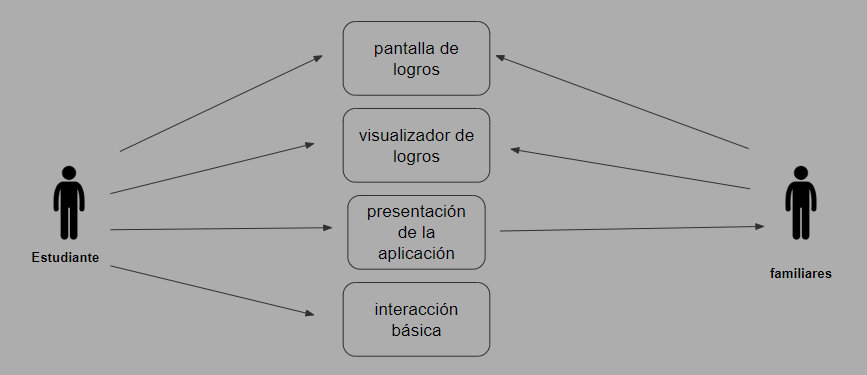
\includegraphics[width=15cm]{imgs/CasoUso_7.PNG}}
\caption{Diagrama de Caso 7}
\label{fig_7_1}
\end{figure}

\paragraph{Modelo Conceptual}

\begin{figure}[H]
\centerline{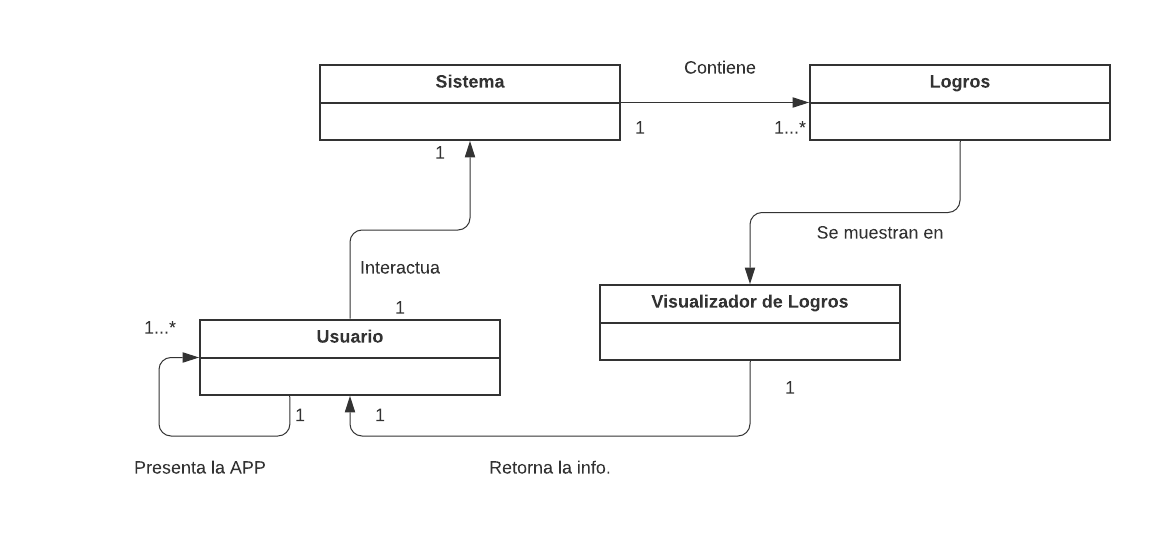
\includegraphics[width=15cm]{imgs/ModeloConceptualCaso_7_3.png}}
\caption{Modelo Conceptual Caso 7}
\label{fig_7_2}
\end{figure}

\paragraph{Diagrama de Secuencia o Colaboración}

\begin{figure}[H]
\centerline{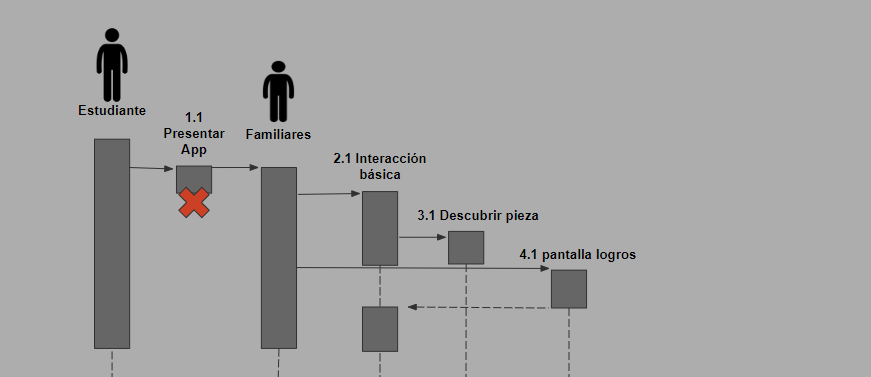
\includegraphics[width=15cm]{imgs/CasoUso_7_2.PNG}}
\caption{Diagrama de Secuencia Caso 7}
\label{fig_7_3}
\end{figure}

\paragraph{Priorización}
{\textbf {Tipo:}}
Deseable.